\sectionquestion{Learning Theory}

\begin{parts}


% Question 4
\part Desmos is a powerful browser-based graphing software. It is so powerful that it can even create this graph of a narwhal; we will call this the special narwhal equation.

    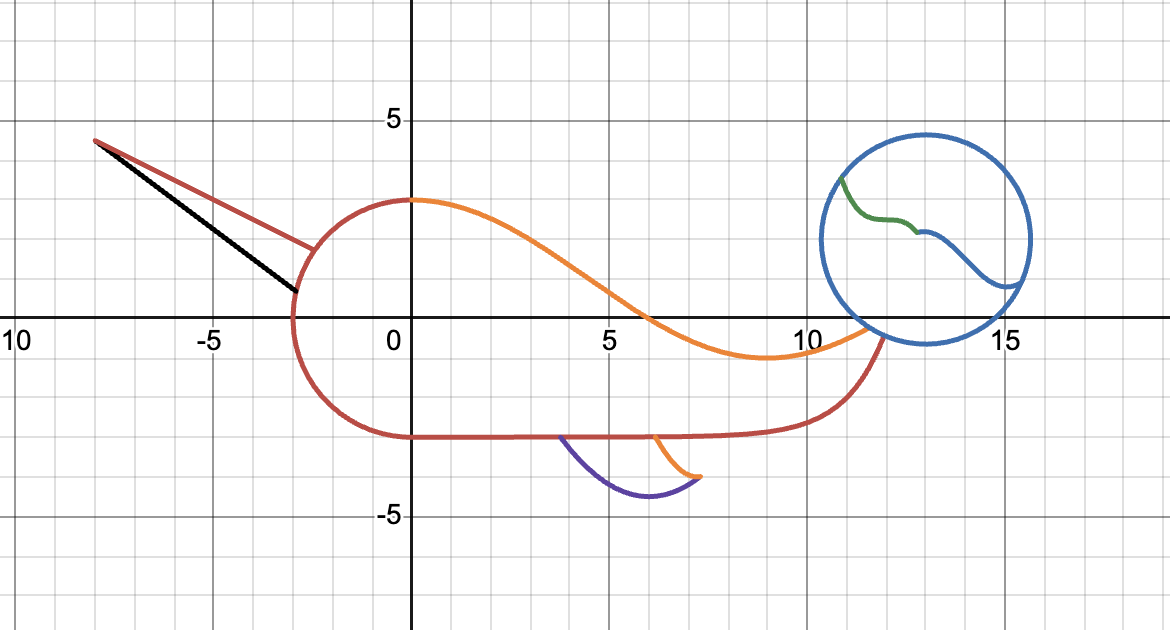
\includegraphics[width=0.5\textwidth]{figures/pac-narwhal.png}
    
\begin{subparts}

\subpart[2] \textbf{Numerical Answer:} We would like to learn the special narwhal equation, but we only know that for a given point, whether it is or is not on the line calculated by the narwhal equation. However, we don't really know where to start, so we try brute-forcing the narwhal equation. We try functions where: 
    \begin{itemize}
        \item The function is a piecewise function with 6 parts.
        \item Each piecewise equation is a polynomial with 5 degrees of freedom.
        \item Each piecewise equation has integer coefficients in the range $[-5, 5)$
        \item Each piecewise equation has an integer upper and lower bound of the interval on which the piece is defined. The lower bound is any integer in the range $[-10, 0)$ and the upper bound is any integer in the range $[0, 10)$.
    \end{itemize}
    How many points do we need to achieve error $\epsilon$ with probability $(1 - \delta)$? \emph{Show your work.} Your final answer can include a $\log$.
    \begin{tcolorbox}[fit,height=5cm, width=15cm, blank, borderline={1pt}{-2pt}]
    %solution
    \end{tcolorbox}
    \begin{soln}
    TODO: double check this answer, it should maybe involve $20^5$?
    
    This falls under the finite and agnostic case. The answer should be that formula, and the $\log(\mathcal{H})$ term should be $\log(6 * 10^6 * 10 * 10)$ = $\log(6 * 10^8)$
    \end{soln}
    \begin{qauthor}
    Emily Xie; Identify the properties of a learning setting and assumptions required to ensure low generalization error, Apply sample complexity bounds to real-world learning examples
    \end{qauthor}

\clearpage
\subpart[1] \textbf{Short Answer:} After discussing with a friend at Desmos, you realize that the VC-dimension of the set of all functions which can be plotted in Desmos is $\infty$ (i.e. this set can shatter datasets of arbitrarily large, finite size). Explain the theoretical implications of this for train error and test error. 
%Assume we gave up and didn't end up finding the special neural equation with the previous method, but since someone managed to make it in Desmos, it must be a Desmos function.
    %First, briefly justify why the VC-dimension of the set of all Desmos functions is $\infty$. Second, 
    \fillwithlines{8em}
    \begin{soln}
    1) The VC-dimension of all Desmos functions is infinity because it can shatter datasets of all sizes (for instance, we can make Desmos directly classify each point in the dataset). 2) There are no bounds or guarantees on the sample complexity and error. This means that no matter how well the train error performs, we will not know if our model can generalize well on a test dataset.
    \end{soln}
    \begin{qauthor}
    Emily Xie; Identify the properties of a learning setting and assumptions required to ensure low generalization error, Apply sample complexity bounds to real-world learning examples

    (adapted by Matt to drop the VC dimension being infinite)
    \end{qauthor}
    
\end{subparts}


% Question 7
\part The inequality below characterizes the relationship between the true error $R(h)$ and the empirical error $\hat{R}(h)$ for any hypothesis $h \in \mathcal{H}$ with VC-dimension $VC(\mathcal{H})$.

\[R(h) \leq \hat{R}(h) + \mathcal{O}\left(\sqrt{\frac{1}{N}\left(VC(\mathcal{H}) + \log(\frac{1}{\delta}) \right)} \right)\]

    \begin{subparts}
    \subpart[1] \textbf{True or False:} Increasing $VC(\mathcal{H})$ always decreases the true error $R(h)$.
    \begin{checkboxes}
     \choice True 
     \choice False
    \end{checkboxes}
    
    \begin{soln}
        False. Although the empirical error $\hat{R}(h)$ does decrease as $VC(\mathcal{H})$ increases, the second term also increases and will overpower the overall bound after a point.
    \end{soln}
        
    \begin{qauthor}
        Emaan Ahmed; Learning Theory: PAC Learning, Distinguish true error, train error, test error.
    \end{qauthor}
        
    \subpart[2] \textbf{Short answer:} $VC(\mathcal{H})$ can be seen as a measure of model complexity. Explain how adding regularization to the model also decreases its VC-dimension. What is the benefit of doing so for model selection?
    \fillwithlines{8em}
    
    \begin{soln}
        The VC-dimension is decreased when we add a regularizer because we effectively reduce the number of features our model considers significant, reducing the model's degrees of freedom. Adding regularization reduces model complexity and thus the risk of overfitting.
    \end{soln}
    
    \begin{qauthor}
        Emaan Ahmed; Learning Theory: PAC Learning, Theoretically justify regularization.
    \end{qauthor}

    % \subpart[2] \textbf{Short answer:} Both the Bias-Variance Tradeoff, which we studied earlier in the semester, and the Approximation Generalization Tradeoff are used to address the risk of overfitting. Identify and explain the factors that lead to an increase in overfitting for each tradeoff.
    % \fillwithlines{8em}
    
    % \begin{soln}
    % BVT: Higher Variance
    
    % AGT: Higher VC-dimension
    
    % Both increase model complexity and lead to overfitting.
    % \end{soln}
    
    % \begin{qauthor}
    % Emaan Ahmed; Learning Theory (PAC Learning): Theoretically justify regularization. Feature Engineering/Regularization: Identify when a model is overfitting 
    % \end{qauthor}
    \end{subparts}


\end{parts}